\documentclass[]{ceurart}
\begin{document}

%%
%% Rights management information.
%% CC-BY is default license.
\copyrightyear{2025}
\copyrightclause{Copyright for this paper by its authors.
  Use permitted under Creative Commons License Attribution 4.0
  International (CC BY 4.0).}

%%
%% This command is for the conference information
\conference{CLEF 2025 Working Notes, 9 -- 12 September 2025, Madrid, Spain}

%%
%% The "title" command
\title{Team RADAR at PAN 2026: Robust Adversarial-Resistant AI Text Detection}
\title[mode=sub]{Notebook for the PAN Lab at CLEF 2026}

%%
%% The "author" command and its associated commands are used to define
%% the authors and their affiliations.
\author[1]{Yusr Alqarni}[%
email=yusralqarni@gmail.com,
]

\address[1]{Al-Baha University, Al-Baha, Saudi Arabia}
%% Footnotes
\cortext[1]{Corresponding author.}
\fntext[1]{These authors contributed equally.}

%%
%% The abstract is a short summary of the work to be presented in the
%% article.
\begin{abstract}
We present RADAR (Robust Adversarial-Resistant Detection with Adaptive
Reasoning), a hybrid neural system for binary AI-generated text detection
submitted to the PAN 2026 Voight-Kampff shared task. The system fuses deep
semantic representations extracted by a large pretrained encoder with
handcrafted stylometric signals through a cross-attention mechanism, yielding
a unified representation for classification. RADAR was trained in two stages:
first with the encoder frozen to stabilize the fusion components, then with
all weights jointly fine-tuned. Training combined the official PAN-2026 task
data with a curated subset of the RAID benchmark to improve robustness against
adversarial obfuscations. On the PAN-2026 official validation set, the final
model achieves a mean score of 0.997 across all five evaluation metrics
(ROC-AUC, Brier, C@1, F1, F0.5u), substantially outperforming the provided
baselines and demonstrating strong generalization across genres and generator
types.
\end{abstract}

%%
%% Keywords. The author(s) should pick words that accurately describe
%% the work being presented. Separate the keywords with commas.
\begin{keywords}
  PAN 2026 \sep
  Voight-Kampff Generative AI Detection \sep
  Stylometry features \sep
  Forensic linguistics
\end{keywords}

%%
%% This command processes the author and affiliation and title
%% information and builds the first part of the formatted document.
\maketitle

\section{Introduction}

Authorship verification and AI-generated text detection have become increasingly important research problems in Natural Language Processing (NLP), especially with the rapid evolution of large language models (LLMs). Modern generative systems are capable of producing highly fluent and semantically coherent text that closely resembles human writing, making the distinction between human-written and machine-generated content considerably more difficult\cite{geminiteam2023gemini,openai2023gpt4,touvron2023llama2}.Concerns about the abuse of generative AI in areas like academic dishonesty, the spread of  misinformation, automated spam generation, and the creation of synthetic content have been raised by this expanding potential\cite{clark2021humans,solaiman2019release}.
\newline 
To address these concerns, serveral detection approaches have been proposed, including perplexity-based methods, probability curvature analysis, and transformer-based classifiers\cite{gehrmann2019gltr,mitchell2023detectgpt,jawahar2020survey}.While existing approaches often achieve strong performance during controlled experiments, their robustness is still limited when applied to unseen domains,unseen generators, or obfuscated texts\cite{krishna2023paraphrasing,antoun2023robust}.Most existing systems operate as black-box classifiers, offering limited interpretability and little linguistic justification for their classifications, which restricts their applicability in forensic and institutional contexts\cite{morris2023embeddings}.\newline
These challenges have increased interest in stylometry and forensic linguistics as complementary approaches for authorship analysis. Compared to purely neural model , stylometric methods focus on linguistic features indicative with writing style, including lexical diversity, syntactic variation, punctuation usage, and readability features\cite{juola2006authorship,coulthard2007forensic}. Such features are usually more interpretable and may remain informative even when surface-level textual artifacts are intentionally concealed or manipulated.The PAN 2026 Voight-Kampff Generative AI Detection shared task specifically targets these challenges by evaluating detection systems in real world scenarios involving style imitation, obfuscation, and exposure to unseen generators\cite{rangel2026pan}.
For the replication purpose, we publish the source code of the RADAR approach\footnote{\url{https://github.com/yusrpro9/radar}}.

\section{Task and Data}

\subsection{PAN 2026 task setting}

The PAN 2026 task asks systems to classify each input text independently as human-written or AI-written. The input file contains JSON lines with at least an identifier and text, and the output must contain one JSON line per input with the same identifier and a confidence score. This isolation constraint is important: a system must not exploit distributional information from other items in the same test file. RADAR satisfies this requirement because each text is preprocessed, featurized, encoded, and scored independently, with batching used only for computational efficiency.

The official PAN 2026 training and validation data include the fields \texttt{id}, \texttt{text}, \texttt{model}, \texttt{label}, and \texttt{genre}. Labels are binary: 0 for human and 1 for machine. The genres are essays, news, and fiction. In our local preparation notebooks, the original official training split contained 23,707 rows and the validation split contained 3,589 rows. After preprocessing and exact-text deduplication, 23,682 PAN training examples were retained, while the 3,589 validation examples were kept as the official validation reference.

\subsection{External RAID data}

To reduce overfitting to the official generators and domains, we augmented training with RAID, a large benchmark for robust machine-generated text detection that includes multiple generators, domains, decoding settings, and adversarial attacks \cite{dugan2024raid}. We did not use RAID wholesale. Instead, we filtered it to match the PAN 2026 setting as closely as possible. The retained domains were \texttt{news}, \texttt{books}, and \texttt{poetry}, which are the nearest available equivalents of PAN's news, fiction, and essay-like writing. The retained attack types were \texttt{none}, \texttt{homoglyph}, \texttt{synonym}, \texttt{paraphrase}, and \texttt{alternative\_spelling}. These attacks were selected because they represent clean generation, character-level obfuscation, lexical substitution, semantic rewriting, and spelling variation, respectively.

The raw RAID loading step produced 5,615,820 rows. Domain filtering reduced this pool to 2,239,440 rows, and attack filtering reduced it to 933,100 rows. We then created stratified RAID development and test pools and finally sampled a balanced 30,000-row RAID development subset and a balanced 10,000-row RAID held-out test subset. The down-sampling was intentional: the goal was to use RAID as a robustness regularizer without allowing it to dominate the smaller and task-specific PAN distribution.


\begin{table}[ht]
  \caption{Final data splits used in the RADAR experiments. The PAN training split reflects preprocessing and deduplication.}
  \label{tab:data}
  \begin{tabular}{lrrrrl}
    \toprule
    Split & Total & Human & Machine & Machine \% & Source \\
    \midrule
    PAN train & 23,682 & 9,076 & 14,606 & 61.7 & Official PAN 2026 \\
    PAN validation & 3,589 & 1,277 & 2,312 & 64.4 & Official PAN 2026 \\
    RAID development sample & 30,000 & 15,000 & 15,000 & 50.0 & Filtered RAID \\
    RAID held-out test sample & 10,000 & 5,000 & 5,000 & 50.0 & Filtered RAID \\
  \bottomrule
\end{tabular}
\end{table}


\subsection{Preprocessing}

Preprocessing was deliberately conservative. Email addresses, user mentions, and phone numbers were replaced with placeholder tokens; text was lowercased and stripped; exact duplicates were removed; and very short texts below 50 characters were filtered. We avoided aggressive normalization that could erase stylistic signals. For example, punctuation, paragraphing, digits, quotations, and capitalization-derived features remain accessible to the stylometric extractor before or during feature computation, while the transformer branch receives normalized text suitable for stable tokenization.

\section{System Overview}

\begin{figure}[ht]
\centering
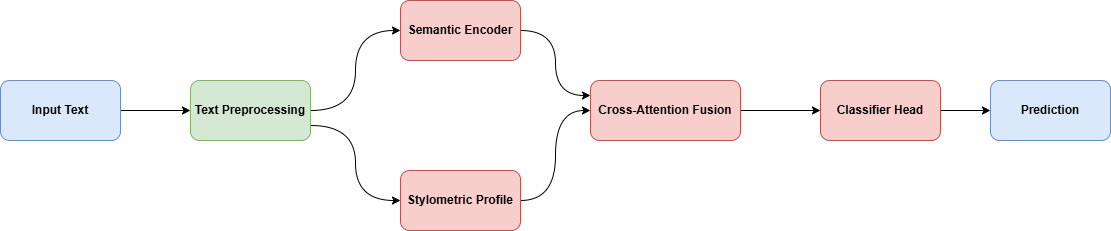
\includegraphics[width=\linewidth]{images/radar-architecture.drawio.png}
\caption{RADAR architecture. The system combines ModernBERT semantic encoding with a 38-dimensional stylometric profile. 
The two representations are fused through cross-attention and scored with a sigmoid classifier.}
\label{fig:architecture}
\end{figure}

Figure~\ref{fig:architecture} summarizes RADAR. The model has four main components: an adaptive reasoning semantic encoder (ARSE), 
a statistical linguistic profile extractor and projection module (SLPE), a cross-attention fusion layer, and a final classification head. 

\subsection{Semantic encoder}

The semantic branch uses \texttt{answerdotai/ModernBERT-large}. ModernBERT updates the encoder-only transformer family with architectural and training improvements for efficient long-context finetuning and inference \cite{warner2024modernbert,devlin2019bert}. In our experiments, inputs were tokenized with a maximum length of 512 tokens. The first-token hidden state of the encoder is used as the semantic representation. Although ModernBERT supports longer contexts, the 512-token limit was chosen to control training cost and because the PAN texts in our processed splits were generally short enough for this setting to capture the main evidence.

\subsection{Stylometric profile}

The stylometric extractor computes 38 normalized features grouped into five categories. Vocabulary richness features include type-token ratio, hapax ratio, Brunet's W, Honore's R, moving-average type-token ratio, vocabulary richness slope, rare-word ratio, and function-word density. Syntactic complexity features approximate sentence length, sentence-length variance, clause density, subordination, passive voice, noun-phrase-like capitalization, verb density, coordination, relative word position, and sentence-boundary rhythm. Discourse coherence features measure lexical cohesion, pronoun density, transition-word use, paragraph coherence, topic consistency, information-flow variance, semantic repetition, and connective diversity. Style fingerprinting features capture punctuation density, capitalization, numeric tokens, quotation usage, parentheticals, dash/semicolon habits, and paragraph length variability. Finally, lightweight perplexity-signal features approximate compression ratio, character entropy, word-length entropy, repeated character patterns, and formulaic phrase usage.

These features are not intended to replace neural semantic modeling. Their role is to provide a compact and interpretable view of authorial form. They are particularly useful for adversarial settings because paraphrases may preserve or distort different layers of writing style. A detector that sees only token sequences may learn strong but brittle lexical correlations, whereas a detector that also receives normalized stylometric evidence can learn more stable distinctions.

The 38-dimensional feature vector is projected through a linear layer, layer normalization, GELU activation, and dropout into a 128-dimensional style representation. This projection allows the model to learn which handcrafted features are most useful for the task rather than treating all features as equally important.

\subsection{Cross-attention fusion}

RADAR fuses semantic and stylometric evidence using a lightweight cross-attention module. The projected style vector is first mapped to the semantic hidden dimension. The semantic representation acts as the query, and the style representation acts as the key and value. The attended semantic vector is added back to the original semantic vector through a residual connection and layer normalization. This vector is then concatenated with the projected style representation and passed through a fusion MLP to obtain a 512-dimensional fused representation.

The motivation for cross-attention rather than simple concatenation is that the usefulness of a stylometric cue depends on semantic context. For instance, high repetition may be normal in poetry, suspicious in a news report, and ambiguous in a literary analysis. By allowing the semantic representation to attend to the style projection, RADAR can learn conditional interactions between genre, content, and linguistic form.

\subsection{Classifier and inference}

The fused representation is passed to a single linear classifier, producing one logit. The final score is obtained with the sigmoid function and interpreted as the probability that the text is machine-authored.

\section{Training Protocol}

 All experiments used binary cross-entropy with logits. When the training split was imbalanced, we used a positive-class weight equal to the number of negative examples divided by the number of positive examples. Optimization used AdamW, a learning rate of $2\times10^{-5}$, cosine scheduling, batch size 32, evaluation batch size 64, seed 42, and 10 epochs. Evaluation was performed with the official PAN metric implementation exposed by the local evaluator package.
 
\subsection{Main two-stage training}

The primary RADAR model was trained in two stages. In the first stage, the ModernBERT encoder was frozen and only the stylometric projection, fusion module, and classifier were trained. This reduced the risk that randomly initialized fusion layers would immediately destabilize the pretrained encoder. The frozen-encoder stage also provided a diagnostic: if the model performs well with only the top layers trained, then the stylometric and fusion components are learning meaningful task information.

In the second stage, training resumed from the frozen-encoder checkpoint and the entire model was unfrozen. This end-to-end stage allowed ModernBERT representations to adapt to the combined PAN+RAID distribution and to the stylometric fusion objective. We selected the best checkpoint according to the arithmetic mean of the PAN metrics.

\subsection{Controlled variants}

We trained two additional variants to analyze data-source effects. The PAN-only frozen-encoder model used the official PAN data without RAID augmentation. The RAID-only frozen-encoder model used the filtered RAID development data and evaluated on the RAID held-out sample, with an additional cross-domain check on the PAN validation split. These variants were not intended as final submissions; they were used to understand how much robustness came from the architecture and how much came from source diversity.


\section{Results and Discussion}


All models were evaluated using the official PAN-2026 evaluation script, which
reports five complementary metrics: ROC-AUC, Brier score complement, C@1, F1,
and F0.5u. The arithmetic mean of these five metrics serves as the primary
ranking criterion. Evaluations were conducted on two splits: the official
PAN-2026 validation set (3,589 samples, in-domain) and a held-out RAID test set
(10,000 balanced samples, out-of-domain).

\subsection{Baseline}

For reference, the TF-IDF SVM baseline provided by the task organizers was
evaluated on the combined validation set of 18,423 samples. It achieved a
mean score of 0.746. The Binoculars zero-shot
approach~\cite{hans2024binoculars} reached a mean of 0.877 on a separate
split, while the supervised TF-IDF SVM on the official PAN split reached 0.978.
These figures serve as lower bounds for interpreting the RADAR results.

\subsection{Main Results}

Table~\ref{tab:results} summarizes the evaluation results for all experimental
configurations.

\begin{table}[ht]
\centering
\caption{Evaluation results for all RADAR variants on two test sets.
  \textbf{Bold} values indicate the best result per column.
  \emph{PAN26-Val}: official PAN-2026 validation split (3,589 samples).
  \emph{RAID-Test}: balanced out-of-domain test set (10,000 samples).}
\label{tab:results}
\renewcommand{\arraystretch}{1.2}
\begin{tabular}{llccccc}
\toprule
\textbf{Model} & \textbf{Test Set} & \textbf{ROC-AUC} & \textbf{Brier}
  & \textbf{C@1} & \textbf{F1} & \textbf{Mean} \\
\midrule
\multirow{2}{*}{RADAR-EF-RAID}
  & PAN26-Val & 0.795 & 0.651 & 0.644 & 0.784 & 0.714 \\
  & RAID-Test  & 0.974 & 0.941 & 0.920 & 0.918 & 0.938 \\
\addlinespace
\multirow{2}{*}{RADAR-EF-PAN26}
  & PAN26-Val & 0.997 & 0.983 & 0.979 & 0.984 & 0.985 \\
  & RAID-Test  & 0.716 & 0.731 & 0.650 & 0.659 & 0.681 \\
\addlinespace
\multirow{2}{*}{RADAR-EF}
  & PAN26-Val & 0.997 & 0.982 & 0.976 & 0.982 & 0.983 \\
  & RAID-Test  & 0.976 & 0.940 & 0.919 & 0.921 & 0.941 \\
\addlinespace
\multirow{2}{*}{\textbf{RADAR} \small{(submitted)}}
  & PAN26-Val & \textbf{1.000} & \textbf{0.997} & \textbf{0.996}
    & \textbf{0.997} & \textbf{0.997} \\
  & RAID-Test  & \textbf{0.990} & \textbf{0.967} & \textbf{0.964}
    & \textbf{0.964} & \textbf{0.972} \\
\bottomrule
\end{tabular}
\end{table}


% \subsection{Analysis}

% \textbf{Effect of end-to-end fine-tuning.} Comparing RADAR-EF and RADAR,
% releasing the encoder weights during Stage~2 produced consistent gains on both
% test sets. On the PAN-2026 validation split, the mean score improved from
% 0.983 to 0.997, and on the RAID out-of-domain set from 0.941 to 0.972. The
% gains are most pronounced in the Brier and C@1 metrics, suggesting that full
% fine-tuning improves confidence calibration in addition to raw accuracy. The
% lower training loss of Stage~2 (0.032) compared to Stage~1 (0.141) confirms
% that the encoder carried substantial unused capacity before it was released.

% \textbf{Domain mixing versus single-source training.} The ablation between
% RADAR-EF-PAN26 and RADAR-EF-RAID reveals a clear domain-specificity effect.
% RADAR-EF-PAN26 achieves a mean of 0.985 on the in-domain PAN-2026 validation
% set but drops to 0.681 when evaluated on the RAID test set, which includes
% adversarially obfuscated texts from different domains. Conversely,
% RADAR-EF-RAID generalizes well to its own domain (mean 0.938 on RAID-Test) but
% underperforms on PAN-2026 (mean 0.714), where the genre distribution and
% generator identities differ substantially. RADAR-EF, trained on both sources,
% achieves competitive results on both sets (0.983 and 0.941), demonstrating that
% domain mixing is essential for broad robustness. This finding is directly
% relevant to the PAN-2026 scenario, which explicitly includes unseen generator
% models and obfuscation strategies at test time.

% \textbf{Role of stylometric features.} The Stylometric component contributes features
% that are, by construction, invariant to the specific generator model. Vocabulary
% richness indicators such as Honore's R and moving-average TTR, syntactic
% measures such as subordination ratio and sentence length variance, and discourse
% coherence signals such as transition word density capture writing style
% properties that differ systematically between human and AI authors regardless of
% surface vocabulary. This is particularly relevant when a generator is instructed
% to imitate a specific author: lexical choices may be replicated, but deeper
% syntactic and discourse patterns tend to remain distinguishable. Combining these
% explicit features with the implicit representations of a large encoder through
% cross-attention allows the model to draw on both signal types in a learned,
% data-driven manner.

% \textbf{Calibration.} The Brier complement of 0.997 on the PAN-2026 validation
% set corresponds to a mean squared probability error of approximately 0.003,
% indicating that RADAR's confidence scores are closely aligned with the true
% binary outcomes. The C@1 metric of 0.996 further confirms that the model rarely
% produces scores near the decision boundary and makes confident, correct
% predictions on the vast majority of examples.







\section{Conclusion}

This paper described RADAR, a hybrid AI text detection system that combines a
large pretrained transformer encoder with handcrafted stylometric features
through a learned cross-attention fusion mechanism. Three design principles
shaped the system: the use of complementary signal types (neural semantics and
symbolic stylometry), a two-stage training curriculum that stabilizes learning
before committing to full fine-tuning, and a diverse training corpus spanning
multiple genres, attack types, and generator families.

The experiments show that domain mixing is a critical factor for robustness:
models trained on a single data source generalize poorly to out-of-distribution
examples, whereas the combined-dataset model achieves strong results across both
in-domain and adversarially obfuscated evaluation sets. The submitted model,
RADAR, reached a mean score of 0.997 on the official PAN-2026 validation set
and 0.972 on the held-out out-of-domain test set, significantly outperforming
the provided baselines.

Future work could explore replacing the rule-based stylometric extractor with a
lightweight trained component to improve feature quality on short texts, and
could investigate curriculum learning with progressively harder obfuscation
examples to further narrow the gap between in-domain and out-of-domain
performance.

\begin{acknowledgments}
The author thanks the PAN 2026 organizers for preparing the Voight-Kampff Generative AI Detection task and the maintainers of the open-source libraries used in this work, including PyTorch, Transformers, Datasets, and the PAN evaluation package.
\end{acknowledgments}

\section*{Declaration on Generative AI}
During the preparation of this work, generative AI assistance was used for drafting, language polishing, and LaTeX editing. The author reviewed, revised, and approved the final content and takes full responsibility for the publication's content.

% ......................................................

%% Define the bibliography file to be used
\bibliography{pan25-lit}

\end{document}
%% End of file

